\documentclass{article}
\usepackage{amsmath,amssymb,graphicx,tikz}
\usepackage{hyperref}
\usepackage{tikz}
\usepackage{amsfonts}
\usepackage{amsmath}
\usepackage{listings}

\title{CSC263 Winter 2016, Assignment 3}
\author{Connor Peet \#1001088208}
\renewcommand{\today}{~}
\hypersetup{pdfpagemode=Fullscreen,
  colorlinks=true,
  linkfileprefix={}}
\begin{document}
\maketitle

\lstset{
    numbers=left
}

\begin{enumerate}
\item [1.]
    \begin{enumerate}
    \item Each node of the AVL tree will contain an integer corresponding to an item in the set $S$. As augmented axillary information it will also contain the sums of all items in its left and right subtrees, or zero if it has no corresponding subtree. A few modifications to \texttt{AVL-Insert(S, i)} to maintain this, none of which alter the worst-case run time of the function:
        \begin{itemize}
        \item If, when running \texttt{AVL-Insert}, we encounter a node that already contains $i$, abort the insertion. Since we're running top-down insertion into a binary tree, if there already exists an $i$ in the tree we are guaranteed to encounter it.
        \item After \texttt{AVL-Insert} is called and before rebalancing, recurse from the new leaf up the tree and update parent nodes' sums. This will do $O(\log n)$ operations (the height of the tree) so will not change the asymptotic complexity.
        \item Rotation functions can be augmented to update nodes' sums as we touch them in constant time: the nodes whose sums may change are the root nodes directly manipulated in the rotation. The sums of their children and the parent node, if any, will not be affected.
        \end{itemize}
    See the figure below for an example tree.

    \begin{figure}[h]
    \centering
    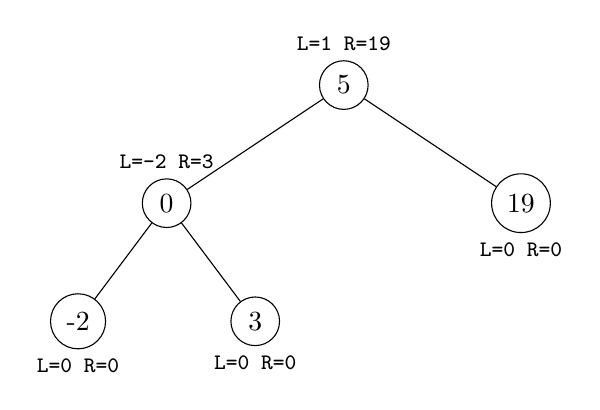
\begin{tikzpicture}[
        level/.style={sibling distance=45mm/#1, level distance = 15mm},
        every node/.style={align=center},
        label distance=0mm,
        every label/.style={text width=20mm, below},
    ]
    \tikzstyle{every label}=[font=\footnotesize]
    \node[circle,draw,label=\texttt{L=1 R=19}]{5}
        child{ node[circle,draw, label=\texttt{L=-2 R=3}]{0}
            child{ node[circle,draw,label=below:\texttt{L=0 R=0}]{-2} }
            child{ node[circle,draw,label=below:\texttt{L=0 R=0}]{3} }
        }
        child{ node[circle,draw,label=below:\texttt{L=0 R=0}]{19} };
    \end{tikzpicture}
    \caption{The resulting tree from $S = \{-2, 0, 3, 19\}$.}
    \end{figure}

    \item Addition has already been described above: it's simply an insertion into the AVL tree. To calculate the sum, one does a standard search on the binary tree, but with a counter initialized to zero. When you traverse down a node add the node's value to the counter, and when you transverse to a right subtree, add the parent's left subtree sum to the counter. When you reach the node, return the value stored in the counter. Because this is just a regular binary search with some constant-time record-keeping at each recursion, it can be expected to run in $O(\log n)$.

\begin{lstlisting}
def sum(T, i, counter=0):
    if T.root == i:
        return T.leftSum + counter
    elif i < T.root:
        if T.left is not None:
            return sum(T.left, i, counter + T.root)
        else:
            return counter
    elif i > T.root:
        if T.right is not None:
            return sum(T.right, i, counter + T.root + T.leftSum)
        else:
            return counter + T.root + T.leftSum
\end{lstlisting}
    \end{enumerate}

\item [2.]
    \begin{enumerate}
    \item [a.] To solve the problem, we'll keep a hash map acting as a set of integers. We insert all $x \in X$ into a hashmap $H$. Then for every $y \in Y$, we'll check if there's any value $z - y_i$ already in the set. If there does exist such an item in the set, we know that $\exists x \in X, z = x + y_i$.

\begin{lstlisting}
def check(X, Y, z):
    H = new Hashmap()
    for x in X:
        H.insert(x, True)

    for y in Y:
        if H.get(z - y) == True:
            return True

    return False
\end{lstlisting}


    \item [b.] The algorithm is fairly simple, running at most $2n$ calls to \texttt{Hashmap.insert} and \texttt{Hashmap.get} in the case that there does not exist an $x$ and $y$ to satisfy the requirements. From the text, the expected running time of insert and retrieval on hashmaps is $O(1)$, therefore the expected running time of this algorithm is in $O(n)$.

    \item [c.] In the worst case the stars align and every integer in $X$ and $Y$ hash to the same key and there is no $x_i + y_j = z$. We end up transversing the linked list at that key, which is of length $n$. The worst-case running time of insertion is still $O(1)$, but the retrieval is $O(n)$. Retrieval run $n$ times on the linked list of size $n$, so the worst-case running time of this algorithm is $O(n^2)$.

    \end{enumerate}
\end{enumerate}
\end{document}
